\documentclass[11pt,letterpaper]{article}
\usepackage[margin=0.86in]{geometry}
\usepackage[T1]{fontenc}
\usepackage[utf8]{inputenc}
\usepackage{lmodern}
\usepackage{xcolor}
\usepackage{tabularx,booktabs,array,longtable}
\usepackage{enumitem}
\usepackage{hyperref}
\usepackage{fancyhdr}
\usepackage{lastpage}
\usepackage{titlesec}
\usepackage{amsmath,amssymb}
\usepackage{microtype}
\usepackage{needspace}
\usepackage{ragged2e}
\usepackage{graphicx}
\definecolor{navy}{HTML}{19334C}
\definecolor{teal}{HTML}{236B82}
\definecolor{soft}{HTML}{EFF5F7}
\definecolor{muted}{HTML}{52616B}
\hypersetup{colorlinks=true,linkcolor=teal,urlcolor=teal}
\titleformat{\section}{\Large\bfseries\color{navy}}{\thesection.}{0.6em}{}
\titleformat{\subsection}{\large\bfseries\color{navy}}{\thesubsection}{0.6em}{}
\titleformat{\subsubsection}{\normalsize\bfseries\color{navy}}{\thesubsubsection}{0.6em}{}
\titlespacing*{\section}{0pt}{15pt}{6pt}
\titlespacing*{\subsection}{0pt}{10pt}{4pt}
\setlength{\parindent}{0pt}
\setlength{\parskip}{4.5pt}
\setlength{\headheight}{15pt}
\renewcommand{\arraystretch}{1.16}
\setlist[itemize]{topsep=3pt,itemsep=2pt,leftmargin=1.4em}
\setlist[enumerate]{topsep=3pt,itemsep=2pt,leftmargin=1.5em}
\pagestyle{fancy}
\fancyhf{}
\fancyhead[L]{\small\color{muted} Applied Machine Learning \textbar{} Cornell Tech}
\fancyhead[R]{\small\color{muted} Human or AI?}
\fancyfoot[C]{\small\color{muted} Page \thepage\ of \pageref{LastPage}}
\renewcommand{\headrulewidth}{0.3pt}
\newcommand{\placeholder}[1]{\par\noindent\textcolor{teal}{\textit{[Your response: #1]}}\par\vspace{0.3em}}
\newcommand{\figplaceholder}[1]{\par\noindent\fcolorbox{teal}{soft}{\parbox[c][1.15in][c]{0.94\linewidth}{\centering\textcolor{muted}{Insert #1 here}}}\par}
\newcommand{\question}[2]{\needspace{4\baselineskip}\par\addvspace{0.45em}\noindent\textbf{#1}\quad #2\par\nobreak\vspace{0.1em}}
\newcommand{\smallnote}[1]{{\small\color{muted}#1}}
\newcolumntype{Y}{>{\RaggedRight\arraybackslash}X}
\makeatletter\newcommand{\tabinput}[1]{\@@input #1 }\makeatother
\newcommand{\commit}[2]{\href{https://github.com/ZhenmanShen/human-or-ai-submissions/commit/#1}{\texttt{#2}}}
\begin{document}
\thispagestyle{empty}
\vspace*{0.2in}
{\color{teal}\bfseries CORNELL TECH \textbar{} APPLIED MACHINE LEARNING}\par
\vspace{0.15in}
{\Huge\bfseries\color{navy} Human or AI?}\par
\vspace{0.07in}
{\LARGE\color{navy} Kaggle Competition Report}\par
\vspace{0.17in}

\textbf{Report Template: }\href{https://www.overleaf.com/project/6ae1fc85355dcf680137d898/share#f2777b20d3adeeecfac9096f78008e2f8daa0ff4be43de3b}{TEMPLATE}

\textbf{Github Repository Template: }\href{https://github.com/sekhari/human-or-ai-submissions}{REPO}

We compared two families of detectors on one fixed 2,000-row validation split. The pretrained track uses features from frozen pretrained language models (GPT-2 token statistics, Qwen2.5 Binoculars scores) and fine-tuned encoders, combined in rank/CDF blends. The classical track trains everything from scratch: TF-IDF n-grams, hand-crafted stylometry and a small Transformer. Three models from each track were submitted to Kaggle. Because held-out training data could not separate the strongest candidates, the final blend was chosen on an out-of-distribution proxy.

\vspace{0.06in}
\begin{tabularx}{\linewidth}{@{}>{\bfseries}p{1.58in}Y@{}}
Team / members & [TODO: names and NetIDs] \\
Kaggle team name & [TODO: Kaggle team name] \\
GitHub PR URL & [TODO: PR URL] \\
\end{tabularx}
\vspace{0.06in}
\subsection*{Your data}
\begin{tabularx}{\linewidth}{@{}lrrY@{}}
\toprule
\textbf{File} & \textbf{Rows} & \textbf{Labels} & \textbf{Purpose} \\
\midrule
\texttt{train.csv} & 10,000 & Visible & Supervised model development: 5,000 human (0), 5,000 AI (1) \\
\texttt{unlabeled.csv} & 3,000 & Hidden & Optional input for semi-supervised methods; required experiment \\
\texttt{test.csv} & 3,000 & Hidden & Predict the probability of AI authorship for Kaggle \\
\texttt{train\_starter\_2000.csv} & 2,000 & Visible & Convenient subset of \texttt{train.csv} for quick experiments \\
\bottomrule
\end{tabularx}

\smallnote{The starter data is a subset, not 2,000 additional labeled examples. Passages are approximately 75--350 words, with mean length near 210 words.}

\subsection*{How the test set works}
The test set mixes familiar and unfamiliar writing domains and AI generators, and includes some adversarially modified AI-written passages. You will \emph{not} receive labels, source model names, domain labels, or difficulty memberships for individual test examples. Submit a probability in $[0,1]$ for each test ID, where 1 means AI-generated. Kaggle evaluates submissions using \textbf{area under the ROC curve (AUROC)}. The \textbf{public leaderboard} covers 900 examples (30\%); the \textbf{private leaderboard} covers 2,100 (70\%) and determines the final competition performance score.

\vfill
\newpage
\section{Competition rubric and submission instructions}
\smallnote{Rubric and instructions as in the official template (Kaggle 25, model comparison 15, data size 10, unlabeled data 5, generalization 20, open-ended 15, code/PR 10). Validation protocol used throughout: fixed stratified 2,000-row split of \texttt{train.csv}, seed 20261023 (\texttt{common/val\_ids.csv}); all models train on the remaining 8,000 rows.}

\section{Team information and model summary}
\question{Q0.1 [0 points].}{List team members and their main contributions.}
[TODO: names, NetIDs and contributions.] Code, experiments and the first draft of this report were produced with Claude Code (see Q6.3).

\question{Q0.2 [0 points].}{Summarize your final approach in 3--5 sentences. What is the overall pipeline from raw text to probability?}
The final submission (blend A) scores each passage with seven models:
\begin{itemize}
\item three LightGBM heads on frozen-LM token statistics plus 43 style features (GPT-2-medium; Binoculars with Qwen2.5-0.5B and -1.5B);
\item one GPT-2 head on token statistics only;
\item three fine-tuned encoders: RoBERTa-base, DeBERTa-v3-large, and the OpenAI GPT-2-output detector (RoBERTa-large).
\end{itemize}
Each model's score is mapped through the empirical CDF of its own out-of-fold training scores, and the final probability is the weighted mean of these percentiles, with weights 3, 3, 2, 1, 1, 1, 1.

The weights were chosen by greedy selection on a held-out proxy: AI text from seven unseen generators plus held-out human poetry and fiction. Cross-validation on train could not separate the candidates.

Our best model trained entirely from scratch, a LightGBM on 101 stylometric features, is 0.0016 behind on validation. It trains in 7 seconds on a CPU.

\question{Q0.3 [0 points].}{Record your final scores (enter private score only once it is revealed).}
\begin{tabularx}{\linewidth}{@{}Yp{1.8in}@{}}\toprule Metric & Your score \\ \midrule Validation AUROC (blend A, fixed 2,000 rows) & 0.99990 \\ Kaggle public AUROC & 0.99161 \\ Kaggle private AUROC & [TODO: after reveal] \\ \bottomrule\end{tabularx}

\newpage
\section{Model comparison and selection (15 points)}
\textbf{Learning goal:} demonstrate sensible representation choices, comparisons of at least three approaches, appropriate hyperparameter selection, and evidence-based selection of the final classifier.

\question{Q1.1 [3 points].}{How did you preprocess and represent the text? Specify tokenization, normalization, word/character features or embeddings, and any feature extraction choices. Why?}
We do no normalisation in either track: case, spacing, line breaks and Unicode are kept. Formatting carries signal: removing it costs every model we tested (Q5).

Representations, from cheapest to most expensive:
\begin{itemize}
\item \textbf{C1:} word 1--2-grams (sklearn regex tokenizer \cite{sklearn}) and character 2--5-grams within word boundaries, sublinear TF-IDF, vocabulary fit on the training rows.
\item \textbf{C2:} 101 closed-form stylometric measurements, partly following Ma et al.\ \cite{ma2023}: sentence-length burstiness, type--token ratio, repetition, punctuation and function-word rates, readability, blank lines and line structure, zero-width and homoglyph counts. Classified with LightGBM \cite{lightgbm}, as are the LM-feature heads.
\item \textbf{C3:} a 12k byte-level BPE tokenizer \cite{bpe} that we trained on the training rows and \texttt{unlabeled.csv}, which keeps spaces and newlines, feeding a small Transformer encoder \cite{transformer} trained from random initialisation.
\item \textbf{Pretrained features:} GPT-2 and GPT-2-medium \cite{gpt2} and Qwen2.5 \cite{qwen25}, each with its own tokenizer (512 tokens), summarised by statistics of token log-probability, rank and entropy. The Binoculars score \cite{binoculars} adds a base/instruct cross-perplexity ratio. These features measure how predictable the text is to an LM, which transfers across topics.
\item \textbf{Fine-tuned encoders:} RoBERTa-base \cite{roberta}, DeBERTa-v3-large \cite{debertav3} and OpenAI's GPT-2-output detector \cite{solaiman2019}, loaded with Hugging Face Transformers \cite{hftransformers}, read sub-word tokens end to end.
\end{itemize}

\question{Q1.2 [5 points].}{Which \textbf{three or more} modeling approaches did you try? Keep the labeled validation partition fixed across models.}
The six models we submitted to Kaggle, three per track, all on the same 8,000 / 2,000 split (seed 20261023):

{\small\begin{tabularx}{\linewidth}{@{}>{\RaggedRight}p{0.9in}Yrrrr@{}}\toprule
Model & Text representation & Train AUROC & Val. AUROC & Train time & Kaggle public \\ \midrule
\tabinput{../common/tables/six_models_q12.tex}
\bottomrule\end{tabularx}}
\smallnote{Train time is one fit on the 8,000 rows; blends sum their members' times. Blends ran on an RTX 5070 and an RTX 3060 (DeBERTa-v3-large); their LM members read cached LM features, so the times exclude feature extraction (1.3--30 min per LM in the original 5-fold runs). C1 and C2 ran on a Ryzen 5 9600X CPU, C3 on the RTX 5070. Classical public scores: [TODO once uploaded].}

\begin{center}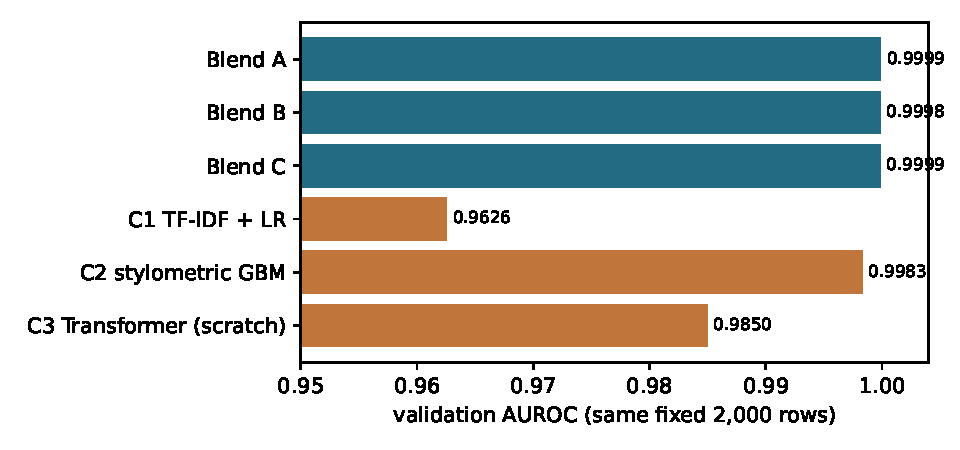
\includegraphics[width=0.49\linewidth]{../common/figures/six_models.pdf}\hfill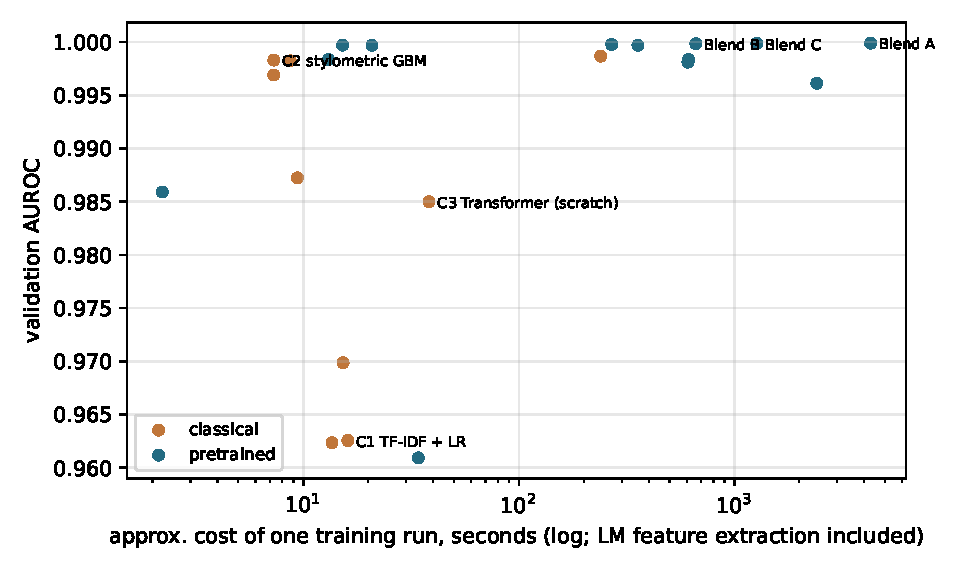
\includegraphics[width=0.49\linewidth]{../common/figures/cost_vs_auroc.pdf}\end{center}
\smallnote{Right: cost of one training run (log scale; LM feature extraction added back for pretrained models) against validation AUROC. The scatter also shows every other model we validated. Their individual numbers, and the 5-fold CV figures from development, are in \texttt{common/results/compare\_tracks.csv} and Appendix A.}

\question{Q1.3 [4 points].}{For at least \textbf{two} approaches, which hyperparameters and candidate values did you try? How did you select the final settings without using Kaggle test labels?}
{\small\begin{tabularx}{\linewidth}{@{}p{0.85in}Yp{1.85in}@{}}\toprule Model & Parameters/values searched & Chosen setting \\ \midrule
\tabinput{tables/q13_hpsearch.tex}
\bottomrule\end{tabularx}}
\smallnote{\texttt{tfidf\_lr} = C1, \texttt{stylo\_gbm} = C2; \texttt{lm\_gpt2} is the LightGBM head on GPT-2 token statistics that blends B and C contain.}

\textbf{Protocol.} Each setting was scored by 5-fold stratified cross-validation inside the 8,000 training rows only; the 2,000 validation rows are in no fold. The best mean fold AUROC wins. Validation was used once afterwards, to report the chosen setting, and never to choose. The pretrained fine-tunes kept fixed epochs, and C3's epoch count was set by early stopping on a 10\% inner split of its training rows.

\textbf{What the searches showed.}
\begin{itemize}
\item TF-IDF prefers weak regularisation and keeping case. C = 64 is the edge of the grid, but only +0.0004 over C = 16.
\item C2 and the LM head are flat across their grids (0.9979--0.9981 and 0.9990--0.9992), so their remaining error is not in the hyperparameters.
\end{itemize}

\question{Q1.4 [3 points].}{Which approach did you choose for your final submission? Explain using validation performance, computational cost and/or stability. If you later changed the model, explain why.}
\textbf{Final choice: blend A.} Validation could not justify choosing between the blends: A, B and C score 0.99990, 0.99985 and 0.99987, differences far below what 2,000 rows resolve. We therefore chose on the out-of-distribution proxy (Q5), where A scored 0.9928 against 0.9906 for B and 0.9910 for C. The public leaderboard agreed: 0.99161 against 0.98848 and 0.98845.

\textbf{Cost.} A is the most expensive submission: about 54 GPU-minutes of fine-tuning plus LM feature extraction. B uses only frozen LMs and would be the fallback if cost mattered.

\textbf{The from-scratch alternative.} Among the classical models, C2 is clearly best: 0.99831 against 0.98500 for C3 and 0.96256 for C1. It is also stable (inner-CV fold standard deviation 0.0005) and the cheapest model we have (7 s on a CPU). It sits 0.0016 below A on validation. How it compares on test, where domains and generators shift, is [TODO: C1--C3 public scores]. Submission history: Appendix A.

\section{Effect of training data size (10 points)}
\textbf{Learning goal:} understand the effect of the number of labeled examples on fitting and generalization. This is an empirical exercise; no formal sample-complexity theory is required.

\question{Q2.1 [4 points].}{Choose one model configuration. Train it with 500, 1,000, 2,000, 5,000 and 8,000 examples sampled from your 8,000-row training partition. Keep the same validation set and hyperparameters.}
Configuration: C2 with its chosen hyperparameters. Subsets are nested and stratified (seed 20261023), and the validation set is fixed. C1 is shown as a contrast in the Notes column. We also ran the same curve for the pretrained \texttt{lm\_gpt2} model (right-hand figure in Q2.2).

\begin{tabularx}{\linewidth}{@{}rrrY@{}}\toprule Training rows & Training AUROC & Validation AUROC & Notes (optional) \\ \midrule
\tabinput{../classical/reports/tables/q21_curve.tex}
\bottomrule\end{tabularx}
\question{Q2.2 [3 points].}{Insert a plot of training and validation AUROC versus training-set size.}
\begin{center}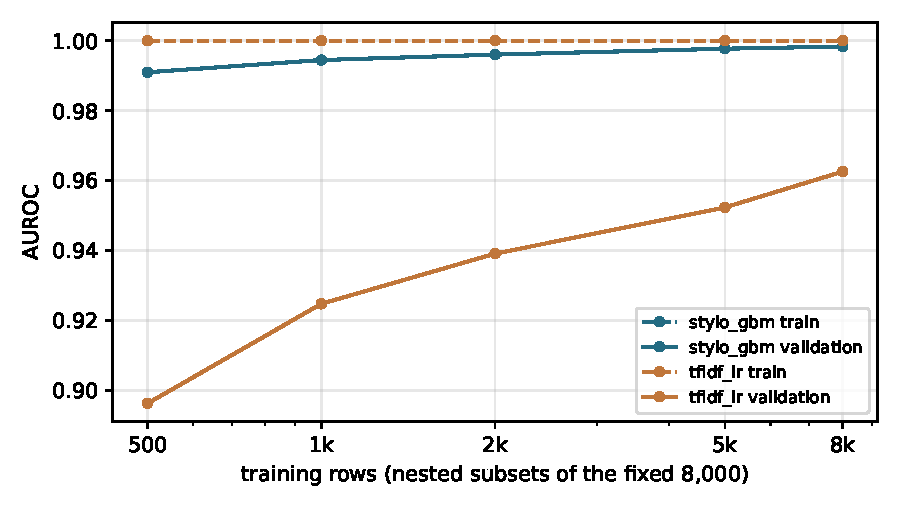
\includegraphics[width=0.49\linewidth]{../classical/reports/figures/learning_curve.pdf}\hfill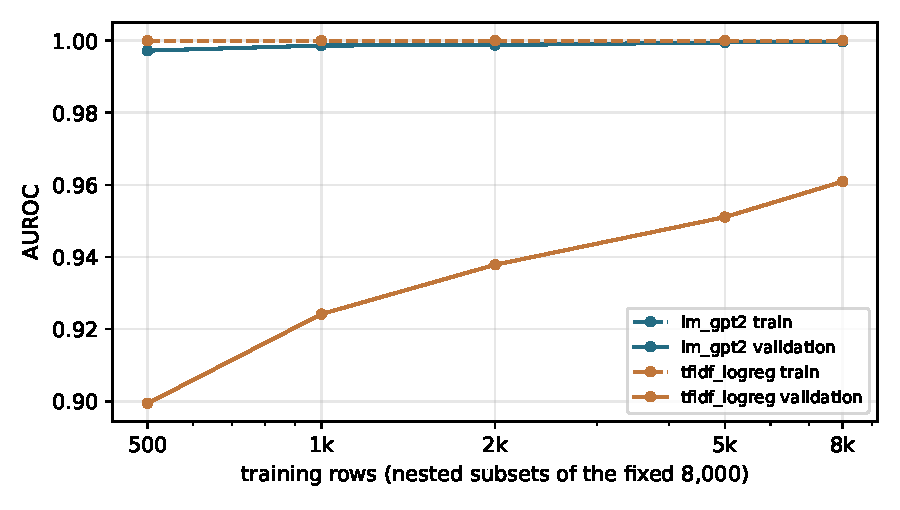
\includegraphics[width=0.49\linewidth]{../pretrained/reports/figures/learning_curve.pdf}\end{center}
\smallnote{Left: C2 (stylometric GBM) and C1 (TF-IDF LR), from scratch. Right: \texttt{lm\_gpt2} (pretrained GPT-2 features) and a TF-IDF LR baseline.}
\question{Q2.3 [3 points].}{What does the curve suggest about overfitting, underfitting, and the value of more labeled examples?}
\textbf{No underfitting, and training AUROC is uninformative.} Training AUROC is 1.000 at every size for C1, C2 and \texttt{lm\_gpt2}. All three separate any training set this small perfectly, so only the validation curves tell us anything.

\textbf{The representation decides how many labels are needed:}
\begin{itemize}
\item \texttt{lm\_gpt2} reaches 0.9972 with only 500 examples. The pretrained LM supplies the representation, and labels only calibrate a small head.
\item C2 starts at 0.9910 and gains about 0.002 per doubling, to 0.9983. A hundred well-chosen features need few examples.
\item C1 starts at 0.896 and gains about 0.015 per doubling. It is still rising at 8,000 rows, the high-variance curve of a 600k-feature sparse model.
\end{itemize}

\textbf{Value of more data.} More labels of the same kind would help C1, but would do little for C2 or the LM features. Test differs from train in domain and generator, so more \emph{diverse} labels (verse, new generators) would plausibly matter more. That is a hypothesis we could not test with the data available.

\section{Learning from unlabeled data (5 points)}
\textbf{Learning goal:} test whether the additional 3,000 unlabeled passages help.
\question{Q3.1 [2 points].}{Describe one method that uses \texttt{unlabeled.csv} (e.g., self-training, confidence-based pseudo-labeling, clustering, or feature learning). How did you prevent validation-label leakage?}
\textbf{Method:} confidence-based pseudo-labelling, also called self-training, with the chosen hyperparameters held fixed.
\begin{enumerate}
\item Train on the 8,000 rows and score \texttt{unlabeled.csv}.
\item Label the 20\% highest-scored passages AI and the 20\% lowest human (1,200 pseudo-labels).
\item Retrain on the 8,000 rows plus the pseudo-labels.
\end{enumerate}
We ran 1 and 3 rounds; each round re-selects pseudo-labels from the newest model. We tested \texttt{lm\_gpt2} and C1/C2.

\textbf{Leakage control:}
\begin{itemize}
\item The pool is \texttt{unlabeled.csv} only: no test or validation text.
\item The validation rows are split off before anything is fit and are scored once, at the end.
\item No unlabeled passage is identical to a validation passage (0 matches).
\end{itemize}
\question{Q3.2 [2 points].}{Compare against a supervised baseline under the same held-out validation protocol.}
\begin{tabularx}{\linewidth}{@{}Yp{1.5in}@{}}\toprule Method & Validation AUROC \\ \midrule
\tabinput{tables/q32_semisup.tex}
\bottomrule\end{tabularx}
\question{Q3.3 [1 point].}{Did it help? Give a concrete, evidence-based explanation (including possible noise in pseudo-labels).}
No. Every change is within $\pm$0.0006, and most are within $\pm$0.0001.

\textbf{Why:} the selected pseudo-labels are passages the model is already certain about.
\begin{itemize}
\item C2: every selected passage scored at least 0.99996 (AI) or at most 0.0001 (human).
\item \texttt{lm\_gpt2}: every selected passage was at least 0.9995 or at most 0.0005.
\end{itemize}
Such examples add no information, and any wrong ones are confirmed rather than corrected. Noise in the pseudo-labels is not the problem here; uninformativeness is.

\textbf{The pool cannot fix the shift either.} \texttt{unlabeled.csv} follows train's mix of forms: 1.2\% verse-like passages, against 16.6\% in test (\texttt{common/results/split\_profile.csv}). It cannot teach the shift that test brings.

\newpage
\section{Generalization and error analysis (20 points)}
\textbf{Learning goal:} characterize how well the selected model generalizes and where it fails. Use \textbf{labeled validation data}; hidden test labels and hidden domain/generator information are unavailable.

\question{Q4.1 [5 points].}{Compare training and validation AUROC for your final selected model. Is there a gap? What explanations are plausible?}
\textbf{Blend A.} Training AUROC 1.00000 (0.999997), validation 0.99990: a gap of 0.0001. At a 0.5 threshold it misclassifies 9 of 2,000 validation passages (3 false positives, 6 false negatives).

\textbf{From-scratch C2.} Training 1.00000, validation 0.99831: a gap of 0.0017, with 7 false positives and 19 false negatives. This is ordinary overfitting of 800 boosted trees, and its inner-CV estimate (0.9981) matches validation.

\textbf{Why the in-distribution gap is small.} The pretrained features do not depend on the labels, and the training distribution is well sampled.

\textbf{The gap that matters is to test.} Blend A drops from 0.99990 on validation to 0.99161 on the public leaderboard. The likely cause is distribution shift: test has unseen generators and far more verse (16.6\% of passages, against 1.6\% of training rows). The out-of-distribution proxy shows every model is weaker on such text (Q5). Validation comes from the training distribution and cannot show this.

\question{Q4.2 [5 points].}{Evaluate performance over at least three text-length bins (define the bins), or another observable subgroup available in your data. Explain why you chose the grouping.}
Blend A (final model), with C2 for comparison:

\begin{tabularx}{\linewidth}{@{}Yrr@{}}\toprule Subgroup / bin (blend A) & Count & Validation AUROC \\ \midrule
\tabinput{../pretrained/reports/tables/q42_subgroups.tex}
\midrule
\multicolumn{3}{@{}l}{\textit{C2 (stylometric GBM), same rows}} \\
\tabinput{../classical/reports/tables/q42_subgroups.tex}
\bottomrule\end{tabularx}

\textbf{Groupings.}
\begin{itemize}
\item Word-count bins: $<$150, 150--250 and $>$250 words. Per-word rates and averaged LM statistics are noisier for short texts and may drift for long ones.
\item Line structure: verse ($\ge$4 lines, median $\le$10 words per line, no digits), short-line lists and recipes, and prose. We chose this grouping because test is 16.6\% verse and C2 leans on layout.
\end{itemize}

\textbf{Results.}
\begin{itemize}
\item Blend A is at or above 0.9998 in every group.
\item C2 is weakest on long passages (0.9967) and on short-line lists (0.9974).
\item Verse is perfect for both models, but rests on only 25 rows (4 AI) and is not informative.
\end{itemize}
This is itself a finding: the subgroup that matters most for test is almost absent from the labelled data.

\question{Q4.3 [5 points].}{Analyze at least \textbf{five false positives and five false negatives} from your held-out validation set. Provide example IDs, predicted probabilities, and short failure hypotheses. Do not paste full passages unless essential.}
{\small\begin{tabularx}{\linewidth}{@{}p{0.5in}p{0.82in}p{0.42in}Y@{}}\toprule ID & Error type & P(AI) & Possible reason \\ \midrule
\tabinput{../pretrained/reports/tables/q43_errors.tex}
\bottomrule\end{tabularx}}
\smallnote{Threshold 0.5 on blend A's score (weighted mean of member percentiles). Blend A makes only 3 false positives at 0.5, so the two highest-scored humans below 0.5 are added as near misses. C2's ten most confident errors are listed in \texttt{classical/results/experiments/fp\_fn\_stylo\_gbm.csv}.}

\question{Q4.4 [5 points].}{What recurring failure patterns did you identify, and how might you address one of them? Distinguish observed patterns from speculation.}
\textit{Observed:}
\begin{enumerate}
\item \textbf{Blend A's errors are disagreements, not confident mistakes.} Every error scores between 0.48 and 0.58. On passages 2696 and 2914, DeBERTa ranks them at 0.87 and 0.05, while the Binoculars and GPT-2-medium members sit at 0.52--0.56.
\item \textbf{The false negatives copy scraped-web layout.} Four of blend A's five false negatives are AI passages formatted like scraped web text: recipe ingredient lines, a Wikipedia hatnote with \texttt{[1]} citations, arXiv-style hard line wraps, bullet glyphs. The same pattern dominates C2's confident false negatives (P(AI) $\le$ 0.006), and two passages (1602, 7049) are errors of both models.
\item \textbf{The false positives are formal, predictable human prose:} news, encyclopedia entries, generic reviews.
\end{enumerate}

\textit{Speculation:} the human training text was scraped, so its formatting artefacts became ``human'' cues that AI text written in that style exploits. Predictable human prose has the low perplexity that LM features associate with AI. One C2 false negative (5316, a fluent but factually invented biography) shows that style alone cannot catch content errors.

\textit{A fix to test:} augment the AI training passages with scraped-web formatting (citation markers, hard wraps, bullets), so that formatting stops implying ``human''. Then measure the shared false negatives and the proxy.

\newpage
\section{Open-ended improvements and insights (15 points)}
\textbf{Learning goal:} propose and test one improvement beyond the required baseline comparisons. This can be simple: a targeted feature change, alternate regularization scheme, ensemble, different representation, augmentation, or training approach. Sophistication alone does not earn credit.

\question{Q5.1 [3 points].}{What specific question or hypothesis motivated your improvement? What weakness or opportunity did you observe?}
\textbf{The weakness.} After a 35-job benchmark, every reasonable model scored at least 0.990 in 5-fold cross-validation. The best dozen runs lay within 0.0005 of each other (fold standard deviation about 0.0005), so CV could not rank them. Yet test differs from train: it has unseen generators, much more creative writing, and 16.6\% verse-like passages against 1.6\%.

\textbf{Hypothesis.} A held-out set that imitates this shift will rank models and blends differently from CV, and choosing the blend on it will improve the leaderboard score. A secondary question, in the from-scratch track: do the three classical models make different errors, so that blending them helps? And how much of C2's strength comes from layout, the cue most likely to break on verse?

\question{Q5.2 [4 points].}{What exactly did you change? Describe the baseline, the new approach and what you held fixed for a fair comparison.}
\textbf{The proxy} (evaluation only, never trained on) combines:
\begin{itemize}
\item 542 rewrites of training human passages and 816 poems and stories, generated locally by seven models never used for training: Llama-3.2-3B-Instruct \cite{llama3}, Qwen3-4B-Instruct \cite{qwen3}, Phi-3.5-mini-instruct \cite{phi3}, SmolLM2-1.7B-Instruct \cite{smollm2}, Granite-3.1-2B-Instruct \cite{granite}, OLMo-2-1B-Instruct \cite{olmo2} and Pythia-1.4B \cite{pythia};
\item 681 human poems and stories from held-out Project Gutenberg books \cite{gutenberg}.
\end{itemize}
\texttt{proxy\_auc} pools these with out-of-fold training scores, weighted so that 41\% is creative writing, like test. Each passage is scored only by fold models that never saw its source.

\textbf{Baseline:} blend B, an equal-weight blend of the four best LM-feature models, chosen without the proxy.

\textbf{New approach:} blend A, chosen by greedy forward selection with replacement \cite{caruana2004} on \texttt{proxy\_auc} over the 18 out-of-distribution-evaluated models and their variants.

\textbf{Held fixed:} the trained models, the CDF blending rule and the training data.

\textbf{Secondary, from scratch:} C2 alone against a C1+C2+C3 blend. The blend's weights come from greedy selection on 5-fold out-of-fold predictions inside the 8,000 rows, with the members' hyperparameters fixed. We also ran ablations of C2 without its 8 layout features.

\question{Q5.3 [4 points].}{What were the measured results?}
{\small\begin{tabularx}{\linewidth}{@{}YrrY@{}}\toprule Configuration & Val. AUROC & Runtime & Relevant difference \\ \midrule
\tabinput{../pretrained/reports/tables/q53_improvement.tex}
\midrule
\tabinput{../classical/reports/tables/q53_improvement.tex}
\bottomrule\end{tabularx}}
\smallnote{Validation = fixed 2,000 rows; runtime = fit on the 8,000 rows. Proxy and unseen-generator AUROC are from \texttt{pretrained/experiments/ood\_eval.csv}. Classical blend weights from inner out-of-fold predictions: C2 0.9, C1 0.1, C3 0.0.}

\textbf{Removing formatting cues} (``debiased'' = no blank lines, double spaces, curly quotes, zero-width characters or homoglyphs; ``join\_lines'' = all lines joined):

{\small\begin{tabularx}{\linewidth}{@{}Yrr@{}}\toprule Model, variant & Fixed-split val AUROC & OOD proxy AUROC \\ \midrule
\tabinput{../pretrained/reports/tables/q53_debias.tex}
\bottomrule\end{tabularx}}

\question{Q5.4 [4 points].}{What did you learn? Did the results support the hypothesis? What limits the conclusion, and what would you try next?}
\textbf{The main hypothesis held.} The proxy ranked the candidates differently from CV: the CV-greedy blend was the best on CV (0.99964) but scored only 0.9862 on the proxy. The proxy put A first, and Kaggle agreed (0.99161 against 0.98848). The fixed split could not see any of this: A and B differ by 0.00005 on validation. The proxy was 0.001--0.003 above the public scores, while CV was 0.008--0.011 above.

\textbf{The from-scratch blend helped a little,} +0.0004 AUROC, with TPR at 1\% FPR rising from 0.983 to 0.990. The gain came from the n-gram model; the Transformer got zero weight.

\textbf{Formatting cues are real signal.} Removing them hurt everywhere: on validation, and on unseen generators (stylometric proxy 0.974 $\to$ 0.915). Without its layout features, C2 falls from 0.9983 to 0.9872, and those features carry 50.4\% of its split gain (\texttt{classical/results/stylo\_gbm/importances.csv}).

\textbf{Limits.}
\begin{itemize}
\item The blend selection is in-sample for the proxy, so A's proxy score is optimistic.
\item The proxy's generators and its archaic Gutenberg human text are a guess at test.
\item One comparison on the 900-row public leaderboard is weak evidence.
\item The 0.0004 classical gain is within the noise of 2,000 rows.
\end{itemize}

\textbf{Next:}
\begin{itemize}
\item Select the blend on half of the generators and score it on the other half, to measure the selection optimism.
\item The formatting augmentation from Q4.4.
\item Bootstrap confidence intervals for small gains.
\end{itemize}

\section{Code submission, reproducibility and AI assistance (10 points)}
\textbf{Submission format:} Submit a \textbf{GitHub PR URL} against the course repository. We will inspect the final code and its development history, not just the final snapshot. Do not squash away meaningful intermediate commits before review. Template \href{https://github.com/sekhari/human-or-ai-submissions}{here}.

\question{Q6.1 [5 points].}{Provide the PR URL, the entrypoint for training/evaluation, and the command used to generate \texttt{submission.csv}. State dependencies and random seeds.}
PR: [TODO: PR URL]. All code is in \texttt{submissions/<team>/}; the README there covers setup and every command. We use Python 3.12. Install with \texttt{pip install -r} the track's \texttt{requirements.txt}; the pretrained track needs PyTorch with CUDA 12.8+ for an RTX 50-series GPU. Kaggle CSVs stay outside git and are passed with \texttt{--data-dir} or \texttt{HOA\_DATA\_DIR}.
{\footnotesize\begin{verbatim}
python common/make_split.py                         # verifies the shared validation split
cd classical && python train.py --model stylo_gbm   # search, fit on 8,000, score the 2,000
python train.py --model stylo_gbm --final           # refit on 10,000 -> kaggle_submissions/
python predict.py --model stylo_gbm --out submission.csv
cd ../pretrained && python run_all.py --profile fixed   # fixed split
python run_all.py --profile ood                     # 5-fold models behind the uploads (~4 h, 2 GPUs)
python make_submission.py --run <7 runs> --weights 3 3 2 1 1 1 1 \
       --name final_A_greedy_proxy
\end{verbatim}}
{\raggedright Seeds: 20261023 for the split, the CV folds and every fixed-split experiment. The original 5-fold runs behind the pretrained uploads used seed 42. In a fresh clone, C2's \texttt{--final} and \texttt{predict.py} reproduce the committed file exactly. Blend A, rebuilt from the saved models, matches with Spearman 1.000000; the saved models are not in git. GPU bf16 inference can differ in the last digits.\par}

\question{Q6.2 [3 points].}{Give two or three examples of changes you made during development. Link to relevant commits or PR discussion and briefly explain what the experiments taught you.}
\begin{itemize}
\item \commit{1fc181fef044ef79830a9a0db09f32bc305f38e0}{1fc181f} (full benchmark, 35 jobs): every reasonable model reached 0.990--0.999 CV AUROC. Training-set CV was saturated, so we built the out-of-distribution proxy, \commit{ed4ad2daeabbb6f05fc791791dff0edf34ced42e}{ed4ad2d}. It ranked models differently, and the blend chosen on it won on Kaggle, \commit{77663a46bfcbc667df49d3aeb81d00485319b2f8}{77663a4}.
\item \commit{345aaab6ff162b0dd75461b219afda13866aed63}{345aaab}: the from-scratch Transformer's inner-split AUROC peaks at epochs 6--7, then falls while training loss keeps dropping. With 7,200 passages a 6.4M-parameter model overfits fast, so early stopping on an inner split, not the validation set, is essential.
\item \commit{6fb8406709d375571d760b4d23b11a131c61c44e}{6fb8406} and \commit{3754f3b7f2d07855ff6e01a9ef753e7f575d4698}{3754f3b}: removing layout from C2 costs 0.011 AUROC, and removing formatting cues hurts the pretrained models too. Formatting is real signal, not just an artefact, which is why we kept it.
\end{itemize}

\question{Q6.3 [2 points].}{How did you use AI tools (such as Claude, ChatGPT or Copilot) for code, debugging, analysis or writing? What did you verify or modify yourself?}
[TODO: team to edit.] Claude Code (Anthropic) wrote most of the code in both tracks, ran the experiments on our machines and drafted this report. Every table number is generated by scripts from committed results files. [TODO: what the team verified or changed themselves.]

The out-of-distribution proxy used text generated locally by seven open models and Project Gutenberg books, for evaluation and blend selection only, never as training labels. No external LLM API labelled or scored test passages, and no hidden labels were retrieved. The classical track uses no pretrained weights.

Pretrained weights used by the pretrained track (Hugging Face):
{\small\begin{itemize}
\item \texttt{openai-community/gpt2}, \texttt{openai-community/gpt2-medium} \cite{gpt2}
\item \texttt{Qwen/Qwen2.5-0.5B}, \texttt{Qwen/Qwen2.5-0.5B-Instruct}, \texttt{Qwen/Qwen2.5-1.5B}, \texttt{Qwen/Qwen2.5-1.5B-Instruct} \cite{qwen25}
\item \texttt{FacebookAI/roberta-base} \cite{roberta}, \texttt{microsoft/deberta-v3-large} \cite{debertav3}
\item \texttt{openai-community/roberta-large-openai-detector} \cite{solaiman2019}
\end{itemize}}
{\small\raggedright Generators used only to build the evaluation proxy (no training labels): \texttt{meta-llama/Llama-3.2-3B-Instruct}, \texttt{Qwen/Qwen3-4B-Instruct-2507}, \texttt{microsoft/Phi-3.5-mini-instruct}, \texttt{HuggingFaceTB/SmolLM2-1.7B-Instruct}, \texttt{ibm-granite/granite-3.1-2b-instruct}, \texttt{allenai/OLMo-2-0425-1B-Instruct}, \texttt{EleutherAI/pythia-1.4b}; references in Q5.2.\par}

\textbf{AI policy.} You may use AI assistants for coding, debugging, explanations, brainstorming, and editing. We expect each team to exercise its own judgment, run experiments, check outputs, and understand its submitted approach. Sending the entire assignment to an AI tool and submitting its unverified output without meaningful involvement does not satisfy the objectives of this project. We will use the PR history, reproducible experiments and report together as evidence of engagement. \emph{Commit counts and the presence of AI-generated code are not themselves grading criteria.} Do not fabricate results or retrieve hidden test labels.

\section*{Final submission checklist}
\begin{itemize}[label=$\square$]
\item Final probabilities submitted to Kaggle for every \texttt{test.csv} ID.
\item Completed report, with all required answers, tables, figures and sources, submitted as PDF.
\item GitHub PR linked on the report title page and in the course submission portal.
\item Code and dependencies recreate final predictions (within reasonable numerical tolerance).
\item Relevant experiments and seed/configuration details are recorded.
\item AI-use disclosure is complete; hidden labels were not retrieved externally.
\end{itemize}

{\small
\begin{thebibliography}{99}\setlength{\itemsep}{1pt}
\bibitem{gpt2} A.~Radford, J.~Wu, R.~Child, D.~Luan, D.~Amodei, I.~Sutskever. Language Models are Unsupervised Multitask Learners. OpenAI technical report, 2019.
\bibitem{qwen25} Qwen Team. Qwen2.5 Technical Report. arXiv:2412.15115, 2024.
\bibitem{binoculars} A.~Hans et al. Spotting LLMs With Binoculars: Zero-Shot Detection of Machine-Generated Text. ICML 2024; arXiv:2401.12070.
\bibitem{roberta} Y.~Liu et al. RoBERTa: A Robustly Optimized BERT Pretraining Approach. arXiv:1907.11692, 2019.
\bibitem{debertav3} P.~He, J.~Gao, W.~Chen. DeBERTaV3: Improving DeBERTa using ELECTRA-Style Pre-Training with Gradient-Disentangled Embedding Sharing. ICLR 2023; arXiv:2111.09543.
\bibitem{solaiman2019} I.~Solaiman et al. Release Strategies and the Social Impacts of Language Models. arXiv:1908.09203, 2019 (the GPT-2 output detector).
\bibitem{hftransformers} T.~Wolf et al. Transformers: State-of-the-Art Natural Language Processing. EMNLP 2020 (System Demonstrations).
\bibitem{lightgbm} G.~Ke et al. LightGBM: A Highly Efficient Gradient Boosting Decision Tree. NeurIPS 2017.
\bibitem{sklearn} F.~Pedregosa et al. Scikit-learn: Machine Learning in Python. JMLR 12, 2011.
\bibitem{ma2023} Y.~Ma et al. AI vs.\ Human -- Differentiation Analysis of Scientific Content Generation. arXiv:2301.10416, 2023.
\bibitem{bpe} R.~Sennrich, B.~Haddow, A.~Birch. Neural Machine Translation of Rare Words with Subword Units. ACL 2016.
\bibitem{transformer} A.~Vaswani et al. Attention Is All You Need. NeurIPS 2017.
\bibitem{caruana2004} R.~Caruana, A.~Niculescu-Mizil, G.~Crew, A.~Ksikes. Ensemble Selection from Libraries of Models. ICML 2004.
\bibitem{llama3} Llama Team, AI @ Meta. The Llama 3 Herd of Models. arXiv:2407.21783, 2024 (Llama 3.2 checkpoints).
\bibitem{qwen3} Qwen Team. Qwen3 Technical Report. arXiv:2505.09388, 2025.
\bibitem{phi3} M.~Abdin et al. Phi-3 Technical Report. arXiv:2404.14219, 2024 (Phi-3.5 checkpoints).
\bibitem{smollm2} L.~Ben Allal et al. SmolLM2: When Smol Goes Big. arXiv:2502.02737, 2025.
\bibitem{granite} IBM Granite Team. Granite 3.1 language models (model card, \texttt{ibm-granite/granite-3.1-2b-instruct}), 2024.
\bibitem{olmo2} Team OLMo. 2 OLMo 2 Furious. arXiv:2501.00656, 2025.
\bibitem{pythia} S.~Biderman et al. Pythia: A Suite for Analyzing Large Language Models Across Training and Scaling. ICML 2023.
\bibitem{gutenberg} Project Gutenberg. \url{https://www.gutenberg.org}.
\end{thebibliography}}

\appendix
\section*{Appendix A. Submission and testing history}
Generated from \texttt{submission\_log.csv} (also \texttt{SUBMISSIONS.md}). The log lists every model validated on the fixed split, from both tracks. ``not submitted'' = tested only; ``pending upload'' = file written, score not yet recorded.

{\footnotesize\begin{longtable}{@{}llp{1.7in}lrll@{}}\toprule
Date & Track & Model & Commit & Val AUROC & Kaggle public & Private \\ \midrule\endhead
\tabinput{tables/appendix_submissions.tex}
\bottomrule\end{longtable}}

\end{document}
